\documentclass[11pt]{article}

\oddsidemargin=0.25truein \evensidemargin=0.25truein
\topmargin=-0.5truein \textwidth=6.0truein \textheight=8.75truein

\usepackage{graphicx}
%\usepackage{amsmath}
\usepackage{verbatim}
\usepackage{booktabs}
\usepackage{comment}
\usepackage{hyperref}
\urlstyle{rm}   % change fonts for url's (from Chad Jones)
\hypersetup{
    colorlinks=true,        % kills boxes
    allcolors=blue,
    pdfsubject={ECON-UB233, Macroeconomic foundations for asset pricing},
    pdfauthor={Dave Backus @ NYU},
    pdfstartview={FitH},
    pdfpagemode={UseNone},
    bookmarksopen=false,
%    pdfnewwindow=true,      % links in new window
%    linkcolor=blue,         % color of internal links
%    citecolor=blue,         % color of links to bibliography
%    filecolor=blue,         % color of file links
%    urlcolor=blue           % color of external links
% see:  http://www.tug.org/applications/hyperref/manual.html
}

\usepackage{verbatim}
%\usepackage{booktabs}
\usepackage[small, compact]{titlesec}

% list spacing
\usepackage{enumitem}
\setitemize{leftmargin=*, topsep=0pt}
\setenumerate{leftmargin=*, topsep=0pt}

\usepackage{needspace}
% example:  \needspace{4\baselineskip} makes sure we have four lines available before pagebreak

\renewcommand{\thefootnote}{\fnsymbol{footnote}}

% document starts here
\begin{document}
\parskip=\bigskipamount
\parindent=0.0in
\thispagestyle{empty}
{\large ECON-UB 233 \hfill Dave Backus @ NYU}

\bigskip\bigskip
\centerline{\Large \bf Properties of Pricing Kernels}
\centerline{Revised: \today}

\bigskip
We return to asset pricing models with macroeconomic foundations ---
macro-finance, for short ---
retracing some of the key steps of the last thirty years.
The term macro-finance means
(a)~we're interested in returns on aggregate assets like bonds and equity indexes
and (b)~we'd like to account for those returns with a macroeconomic model,
such as one with a representative agent.

A short summary would go like this:
%
\begin{itemize}
\item Mehra and Prescott (JME, 1985) on the equity premium.
They showed that a representative agent model with power utility
can't account for the observed average excess return on equity
with reasonable risk aversion.
We get the sign right, but not the magnitude.
\item Hansen and Jagannathan (JPE, 1991) traced the problem to the pricing kernel.
The so-called HJ bound shows that the dispersion of the pricing kernel
is bounded below by the Sharpe ratio of any traded asset, including equity.
Therefore the issue with the equity premium has to do with the pricing kernel,
not the dividends to which equity is a claim.
I like a variant of this result, in which dispersion is measured
by entropy, something we'll define when we get to it.
\end{itemize}
%
In short, when we observe high excess returns or Sharpe ratios,
they tell us that there must be a lot of dispersion in the pricing kernel ---
dispersion being here a suitably vague term that we'll define more precisely later on.
Any model lacking such dispersion is dead from the start.
With power utility, that typically means high risk aversion,
which brings us back to what degree of risk aversion is reasonable.
The evident problems with the representative agent power utility model
is the key driving work in this area.  

In all of this, we'll use a timing convention in which $t$ is now
and $t+1$ is later.
With time measured in years, $t+1$ would be one year from now.
That's similar to what we've done so far,
but with $t$ taking the place of date 0 and $t+1$ taking the place of date 1.
The change is superficial, but makes the comparison with data
more natural.


\section{The nature of research}

Lots of people do research:  analysts, academics, etc.
The content varies, but there's a common theme.
Research is about
(i)~asking an interesting question
and (ii)~providing an informative answer.
The route from (i) to (ii) varies, because we never know
what we'll find.
That's why we call it research:
we don't know the answer until we do it,
and sometimes not even then.

So what makes a good question?
Here are some examples to help us think about that:
%
\begin{itemize}
\item What will GDP growth be next year?
That's not a great question.  The only way to resolve it, really,
is to wait and see what happens.
Perhaps we could modify it:
What is our best prediction of next year's GDP growth?
That's a well-defined statistical exercise that we could
imagine making some progress on.
Still not wildly interesting, at least to me,
but it's a step forward.

\item What is the population of the US?
Again, not a great question.
We look up the answer and we're done.
Although a closer look would tell us that we never really know
the population.
The Census attempts to come up with an answer every ten years,
but it's well-known to be an approximation.
Probably a pretty good one, but an approximation.

One the other hand, thinking about the population could lead us
to better questions.
What fraction of the population is above 70?
What fraction has a college education?
What do the answers tell us about how the US economy works?
You get the idea:  even a bad question can get us thinking in a useful way.

\item What have the average returns been on bonds and equity over the last
century?
This is a little more complex, but still in essence a lookup.
We need to collect data on returns and compute sample means.
When we do that, we'll run across some questions about the definitions
of the assets:  what equity?  what bonds?
You can see an example of such an effort in Table 1.
There we've expanded the question to include the standard deviation,
skewness, and excess kurtosis.
%We've also include two definitions of returns:
%growth returns $r$ and log returns $\log r$.
%Which is better? That depends on what we want to do with them.

\item Why is the excess return on equity roughly 4\%?
This one calls for a model.
Can we construct a model that has this feature?
Is it plausible?
This is the question addressed by Mehra and Prescott,
one we'll address ourselves in much the same way they did.

More generally, why do some assets have higher returns, on average, than others?
Should we invest more in them?  Can we make money doing this for others?
Each of these questions has both practical and intellectual interest.
\end{itemize}
%
What questions appeal to you?
What would you like to know more about?
Keep notes, perhaps with links,
and come back to them now and then.
You'll remind yourself how much fun it is to think about new things
and, sometimes, to make progress in your understanding of them.


\section{Properties of excess returns and consumption growth}

We'll start with the evidence on asset returns, 
specifically US assets over the last 100+ years.
We summarize the basic features of such returns in Table 1 and Figure 1.
Table 1 includes some of the properties of
real (inflation-adjusted) returns on equity (the S\&P 500)
and bonds (one-year Treasuries) for the period 1889-2009.
It also includes similar properties of consumption growth,
for reasons that will be clear shortly.

It's clear from Figure 1 that the variation in excess returns on equity
is closely related to variation in aggregate consumption growth.
In that sense, returns are a macroeconomic phenomenon:
returns tend to be high when consumption growth is high.

Beyond this, we have some useful summary statistics.
We compute them in levels of returns ($r^1$ and $r^e$)
and logs ($\log r^1$ and $\log r^e$).
The same with consumption growth:  $g_{t+1} = c_{t+1}/c_t$
and $\log g_{t+1}$.
You might be asking yourself:  Why logs?  
The answer is that it fits nicely with some theory we'll do shortly. 
Which is a reminder:  the concept of an excess return is a definition,
and we get to decide which definition to use.  
If logs are more convenient, then we go back (as we did here)
and compute excess returns in logs.  

Here are the numbers, computed both ways.  
In levels, the mean short or riskfree rate is 2\% ($r^1 = 1.02$).
The mean excess return on equity is 5.7\% ($r^e - r^1 = 0.057$).
For later reference, the {\it Sharpe ratio\/}
is the mean excess return divided by its standard deviation.
(That's another definition, also useful in some contexts.) 
For equity, that's $ 0.0571/0.1873 = 0.3049$.
(That's way too many digits, but I want to be clear about the calculation.)
These numbers, or something like them, are targets for numerical examples
of theoretical models.


Since many of our models are loglinear, we report similar numbers in logs.
In logs, the mean short rate is 1.8\% ($\log r^1 = 0.018$)
and the mean equity premium is about 4.0\% ($\log r^e - \log r^1 = 0.04$).
I've rounded off most of these numbers to keep things simple.

We'll come back to the properties of consumption growth shortly.


\section{The riskfree rate and equity premium puzzles}
\label{sec:equity-premium}

Now the question:  Can we account for the 4\% equity premium we observe in US data?
How would we start?
The question calls for a model, one capable of producing a similar premium.
If we find one, then we have an explanation.
We can then decide whether we find the explanation plausible
or should continue our search for a better model.

We'll start in the obvious place: a representative agent economy
with power utility.
We then give it a realistic distribution of consumption growth
and (this is the short cut) tie dividends to consumption growth.
We can come back later and see if that's a problem.
We're following our own advice here:
keep things as simple as we can.

We'll use two numerical examples to see how this might work.
Both are similar to Mehra and Prescott's original work.
In each case, we can look at the equity premium either in levels or logs.
I prefer logs --- you'll see why shortly --- but we reported the evidence both ways.

{\it Example (Bernoulli).}
Our first example is as simple as they come.
At each date $t$, there are two states at the subsequent date $t+1$.
Call them $ z \in \mathcal{Z} = \{-1, 1\}$ and give each
a probability of one-half, $p(-1) = p(1) = 1/2$.
Then let  log consumption growth $\log g_{t+1} = \log (c_{t+1}/c_t)$ be
\begin{eqnarray*}
    \log g_{t+1}(z) &=& \mu + \sigma z .
\end{eqnarray*}
The good news is that the calculations are relatively easy with two states.
The bad news is that they're opaque.

With this setup, the mean and standard deviation of log consumption growth
are $\mu$ and $\sigma$, respectively.
Looking at Table 1, we use the values $\mu = 0.02$ and $\sigma = 0.035$,
which gives us a distribution we can argue is realistic.

Asset pricing follows from a pricing kernel and the dividends or cash flows
of the relevant assets.
With a representative agent and power utility, the pricing kernel follows
from consumption growth:
\begin{eqnarray*}
    m_{t+1} (z) &=& \beta g_{t+1}(z)^{-\alpha} .
\end{eqnarray*}
The assets of interest are the riskfree bond, which has a dividend of 1 in all states,
and ``equity,'' which has a dividend of $g_{t+1}(z)$ in state $z$.
The riskfree rate is $r^1 = 1/q^1$ where
\begin{eqnarray*}
    q^1 &=& E (m_{t+1} )  \;\;=\;\; \sum_z p(z) m(z) .
\end{eqnarray*}
Let us say that equity is a claim to consumption growth.
Its price is then
\begin{eqnarray*}
    q^e &=& E (m_{t+1} g_{t+1} )  \;\;=\;\; \sum_z p(z) m(z) g(z) .
\end{eqnarray*}
Its return is $ g(z)/q^e$, so its mean return is $E(r^e) = E (g)/q^e$.
The equity premium is $ E(r^e) - r^1$.
In this environment, each of these calculations is easily done in Matlab.

So what do we get?
We set $\beta = 0.99$ to get started.
If $\alpha = 2$, the riskfree rate $r^1$ is 1.0383, which well above our target of 1.020,
and the equity premium 0.0025, which is well below our target of 0.057.
We could fix the riskfree rate by raising $\beta$,
but this has its limits ($\beta \leq 1$?).
If we raise $\alpha$ to 5, the riskfree rate is 1.0995,
which is even higher,
and the equity premium rises only to 0.0067.
If we take this range of $\alpha$ to be reasonable, we're stuck.

We thus have two problems.
One is what is often termed the {\it riskfree rate puzzle\/}:
the short rate is too high.
If we increase $\beta$ to fix this, we end up with $\beta>1$,
which seems implausible.
(And if we extended utility to more periods, we run into technical problems.)
The second problem is the {\it equity premium puzzle\/}:
we haven't reproduced anything close to the equity premium we see in the data.
Would larger values of $\alpha$ work?  Would they be plausible if they did?
It's not clear, but such values do seem outside what we decided earlier
fit our own sense of risk aversion.

[See Matlab program for computations.]


{\it Example (lognormal).}
Our second example is based on a lognormal environment.
The results are similar, but here we get to look at the solutions
and see where they go wrong.
Let us say that $\log g_{t+1} \sim \mathcal{N}(\kappa_1, \kappa_2)$.
That gives us the pricing kernel
$\log m_{t+1} \sim \mathcal{N}(\log \beta - \alpha \kappa_1, \alpha^2 \kappa_2)$.
We'll look at the riskfree rate and equity premium in logs here,
because that fits well with this example.


We'll use a convenient shortcut, which I got from Andy Abel.
Consider a claim to $g_{t+1}^\lambda$.
If $\lambda = 0$, we get the riskfree bond,
and if $\lambda = 1$ we get equity.
Some people refer to $\lambda>1$ as ``levered equity''
because the dividend is more sensitive to changes in output,
as it would be with increased leverage.
The price of this asset is
\begin{eqnarray*}
    q(\lambda) &=& \beta E \left( g_{t+1}^{\lambda-\alpha} \right)
            \;\;=\;\; \beta \exp \left[ (\lambda - \alpha) \kappa_1
                    + (\lambda-\alpha)^2 \kappa_2 /2 \right] .
\end{eqnarray*}
That gives us log returns of
\begin{eqnarray*}
   \log r^1  &=& - \log \beta + \alpha \kappa_1 - \alpha^2 \kappa_2/2 \\
   E (\log r^e ) &=& - \log \beta + \alpha \kappa_1 - (\alpha-\lambda)^2 \kappa_2/2 \\
   E (\log r^e - \log r^1 )
        &=& [ \alpha^2 -  (\alpha-\lambda)^2 ] \kappa_2/2  \\
        &=& \lambda (2 \alpha -\lambda)  \kappa_2/2  \\
        &=& (2\alpha - 1)  \kappa_2/2 \;\; \mbox{ when } \lambda = 1 .
\end{eqnarray*}
We can see both puzzles right here.
The riskfree rate $r^1$ is quadratic in $\alpha$.
At moderate values, it increases with $\alpha$, so the riskfree rate will be too high.
(You can add numbers to make this more precise.)
But if $\alpha$ gets big enough, the impact of the variance term will bring it down again.
In this sense, we can resolve the riskfree rate puzzle by choosing $\alpha$ really large.
The equity premium, on the other hand, is strictly increasing in $\alpha$.
If we make $\alpha$ large enough, we can account for any equity premium we like.
Using $\kappa_1 = 0.035^2 $,
we hit the equity premium of 0.0400 (in logs, remember) at
\begin{eqnarray*}
    2 \alpha - 1 &=& 2 (0.0400) / (0.035^2) ,
\end{eqnarray*}
or $\alpha = 33.15$.

Both examples make the same point:
that we can't account for the observed equity premium unless
we use a large value of $\alpha$.
Is $\alpha = 33$ reasonable?
There's some debate about that,
but our own thought experiment in class suggests it's more than a bit high.
People with that kind of risk aversion won't be willing to take much risk,
which is why it generates a large equity premium.

Where do we go from here?
When other classes have discussed this,
they had a number of good suggestions.
Among them:
(i)~consider a more complex distribution of dividends;
(ii)~ditto consumption growth;
(iii)~use some kind of ``friction'' so that the risks faced by an individual
are greater than those evident in aggregate consumption; and
(iv)~allow different preferences.
All of these are good ideas, but my money's on (iii).
The first one we'll rule out shortly.
The others take more advanced tools than we have at present,
but we may come back to them if we have time.


\section{The Hansen-Jagannathan bound}

If we think of the equity premium as a problem, the question is where its roots lie.
The answer, in large part, is the pricing kernel.
In this section and the next we derive two bounds on the variability of the pricing kernel.
Observed risk premiums give us lower bounds on the variability of the pricing kernel,
whatever it might be.
With power utility, the point is that you need lots of risk aversion to get enough
variability.

The first bound comes from Hansen and Jagannathan.
They note that the return on any asset $j$ satisfies
\begin{eqnarray}
    E \left( m r^j \right) &=& 1 .
    \label{eq:foc}
\end{eqnarray}
If we take two assets, say $j$ and $1$,
then the excess return $x = r^j - r^1$ satisfies
\begin{eqnarray*}
    E \left( m x \right) &=& 0 .
\end{eqnarray*}
That's true for any two returns.

Let's see where this leads.
Expanding terms and applying the definition of the covariance gives us
\begin{eqnarray*}
    E \left( m x \right) &=& E (m) E(x) + \mbox{Cov}(m,x)
            \;\;=\;\; E (m) E(x) + \rho_{mx} \mbox{Std}(m) \mbox{Std}(x) .
\end{eqnarray*}
Here $\rho_{mx}$ is the correlation between $m$ and $x$
and $\mbox{Std}$ is the standard deviation.
Since the absolute value of the correlation is less than one,
we have
\begin{eqnarray}
  \frac{| E(x)|}{ \mbox{Std}(x)} &\leq& \frac{\mbox{Std}(m)}{E(m)} .
  \label{eq:hj-bound}
\end{eqnarray}
This is the HJ bound.
It says that the Sharpe ratio (the left side) places a lower bound
on the dispersion of the pricing kernel.
Dispersion here is the ratio of the pricing kernel's standard deviation to its mean.
The mean is close to one (the price of a one-period bond),
so it's more or less the standard deviation.

We've seen, then, that observed Sharpe ratios place lower bounds
on the dispersion of the pricing kernel.
How do our examples work?
I leave the calculations to you, but both of the examples from the previous
section violate the bound with reasonable values of the risk
aversion parameter $\alpha$.
That means that the problem is in the pricing kernel:
there's no point trying other dividend processes,
they won't solve the problem.


\section{Entropy}

The term {\it entropy\/} has been used in lots of situations, including thermodynamics,
but its modern use in many fields follows from Shannon's
classic application to information theory.
Tom Sargent passed on this wonderful quote:
%
\begin{quote}
When Shannon had invented his quantity and consulted
von Neumann on what to call it, von Neumann replied:
``Call it entropy. It is already in use under that name and,
besides, it will give you a great edge in debates because
nobody knows what entropy is anyway.''
\end{quote}
%
The idea in most applications is that entropy is a measure of dispersion.

We define the pricing kernel's entropy $H(m)$ by
\begin{eqnarray*}
    H(m) &=& \log E(m) - E (\log m) .
\end{eqnarray*}
Since $\log$ is a concave function,
Jensen's inequality assures us that $H(m) \geq 0$,
with equality only if $m$ is constant.
It is, therefore, a measure of dispersion or variability.
Another property:
$H(\lambda m) = H(m)$ for any positive constant $\lambda$.
[Show by applying the definition.]

{\it Example (lognormal)\/}.
Suppose $ \log m \sim \mathcal{N}(\kappa_1,\kappa_2)$.
Then
\begin{eqnarray*}
    H(m) &=& (\kappa_1 + \kappa_2/2) - \kappa_1
            \;\;=\;\; \kappa_2/2 ,
\end{eqnarray*}
the variance over two.

This is not the definition you'll see elsewhere, so let's connect them.
Recall that the pricing kernel is related to risk-neutral
probabilities by $ p m = q^1 p^* $ or $ m = q^1 p^*/p $.
From the properties of $H$, we have
\begin{eqnarray*}
        H(m) &=& H (p^*/p) \;\;=\;\; - E \log (p^*/p) .
\end{eqnarray*}
Here and throughout, the expectation $E$ is based on the true probabilities $p$.
The quantity on the right is referred to as the
{\it relative entropy of $p$ with respect to $p^*$\/}.
If you'd like to know more, let me know and I'll point you to the classic
references.


\section{The entropy bound}

Now that we've defined entropy, we can describe the entropy bound.
It has a different structure from the HJ bound but a similar spirit.

We start again with the pricing relation (\ref{eq:foc}).
If we take the log of $mr$, Jensen's inequality tells us
\begin{eqnarray*}
    E \left[ \log ( m r^j )\right]
        \;\;=\;\; E \left( \log m + \log r^j \right)
        &\leq& \log (1) \;\;=\;\; 0 .
\end{eqnarray*}
Rearranging terms gives us
\begin{eqnarray*}
    E (\log r^j)  &\leq& - E (\log m ). %\;\;=\;\; E \log m^{-1} . %\;\;=\;\; - E \log m.
\end{eqnarray*}
The highest possible mean log return, in other words, is $\log r = - \log m$.


That gives us the second term in entropy, but what about the first?
We have
\begin{eqnarray*}
     \log E (m)  &=& \log q^1 \;\;=\;\; - \log r^1 .
\end{eqnarray*}
Together we have
\begin{eqnarray}
    E  (\log r^j) - \log r^1  &\leq& \log E(m) - E (\log m)  \;\;=\;\; H(m) .
    \label{eq:entropy-bound}
\end{eqnarray}
In words: excess returns place a lower bound on the entropy
of the pricing kernel.
Like the HJ bound, properties of returns give us a lower bound
on the dispersion of the pricing kernel.
Here dispersion is measured by entropy.

Thus properties of returns tell us something about the pricing kernel.
Consider the lognormal case.
If $\log m \sim \mathcal{N}(\kappa_1,\kappa_2)$, then an equity premium (in logs) of 0.04
gives us a lower bound on the variance $\kappa_2$:
\begin{eqnarray*}
    0.0400 \;\;\leq\;\; H(m) &=& \kappa_2/2.
\end{eqnarray*}
With other distributions, entropy incorporates all the high-order cumulants of $\log m$.
Recall that $\log m$ has the cumulant generating function
\begin{eqnarray*}
    k(s; \log m) &=& \log E \left( e^{s \log m} \right) .
\end{eqnarray*}
The first term in the definition of entropy is therefore $k(1; \log m)$.
If the cgf has the power series expansion
\begin{eqnarray*}
    k(s; \log m) &=& \kappa_1 s + \kappa_2 s^2/2 + \kappa_3 s^3 / 3! + \kappa_4 s^4/ 4! + \cdots
\end{eqnarray*}
for some suitable range of $s$,
then
\begin{eqnarray*}
    H(m)  &=& \kappa_2 /2 + \kappa_3 / 3! + \kappa_4 / 4! + \cdots .
\end{eqnarray*}
The first term is the lognormal term.
The others illustrate the potential benefit of departing from normality,
since they can increase entropy even when we hold the variance constant.
Our colleague Stan Zin refers to this as the {\it never-a-dull-moment conjecture\/}:
if a model doesn't work, you can in principle fix it up by adding enough
high-order cumulants.
Whether that's reasonable is another matter, but it's an interesting
illustration of the benefits of going beyond the normal distribution.
Note in particular that positive skewness ($\kappa_3 > 0$) and kurtosis ($\kappa_4 > 0$)
make positive contributions to entropy.


The $\kappa_j$'s here are cumulants of $\log m$,
but with power utility, it's not hard to show that they're connected to cumulants
of $\log g$:
\begin{eqnarray*}
    \kappa_j (\log m) &=& (-\alpha)^j  \kappa_j (\log g), \;\;  j\geq 2.
\end{eqnarray*}
We see that for odd cumulants to make a positive contribution to entropy,
the cumulants of log consumption growth must be negative.
Thus negative skewness in $\log g$ leads to positive skewness in $\log m$.
Amir Yaron notes that the power of $\alpha$ allows small cumulants in log consumption growth
to become large cumulants in the log pricing kernel.
We refer to that as {\it Yaron's bazooka\/} in his honor.

Before finishing, here's a calculation related to the equity premium.
In the lognormal case,
$\kappa_2(\log m) = \alpha^2 \kappa_2(\log g)$.
The bound based on the equity premium therefore implies
\begin{eqnarray*}
    H(m) &=& \alpha^2 \kappa_2(\log g)/2 \;\;\geq\;\; 0.0400 .
\end{eqnarray*}
With $\kappa_2 = 0.035^2 $ (Table 1),
that implies $\alpha \geq 8.08$.
This is lower than our equity premium calculation,
but then it's a lower bound.


%\section{Another take on risk premiums}
%
%****** ???? *****
%
%Derive risk premiums from co-entropy ...


\section*{Bottom line}

The representative agent model has one big strength:
it associates risk premiums with the cyclical behavior
of output, profits, and dividends, which seems roughly right.
Put simply: Assets that pay off most in good times, when consumption is high, 
have positive risk premiums. 
The numbers, however, are off.
The equity premium, the Hansen-Jagannathan bound, and the entropy bound
all point to variability of the pricing kernel as the key issue for asset pricing models.
Representative agent models with plausible degrees of risk aversion simply don't generate
enough variability to account for the equity premium --- and, presumably,
lots of other assets with nonzero risk premiums.

Perhaps for this reason, financial professionals often
use arbitrary pricing kernels designed to fit a set
of asset prices well.
These models don't tell us where risk premiums comes from,
but they approximate observed asset prices reasonably well.
We'll see examples of this kind of thing when we turn to option and bond pricing.


\section*{Practice problems}

\begin{enumerate}

\item {\it Equity premium with Bernoulli consumption growth.\/}
We work through a bunch of the computations from this chapter
in a simple setting to make sure we understand how they work.
We'll use the Bernoulli example from Section \ref{sec:equity-premium},
where  $ z $  takes on the values $\{-1, 1\}$ with probabilities $\{ 1/2, 1/2 \}$.
Log consumption growth is $ \log g(z) = \mu + \sigma z$.
Assets are valued by a representative agent with power utility,
risk aversion parameter $\alpha = 5$, and discount factor $\beta = 0.99$.

\begin{enumerate}
\item Use the values in the text for $\mu$ and $\sigma$.
What is their rationale?
\item What are the values of the growth rate $g$ in each state?
\item What values does the pricing kernel take in each state?
\item What is the riskfree rate with these values?
\item Define equity as a claim to the growth rate $g$.
What is its price?
Its return in each state?
\item What is the equity premium in levels?
What is equity's Sharpe ratio?
\item What are the mean and variance of the pricing kernel $m$?
What is the maximum Sharpe ratio this economy can generate?
\item What is the equity premium in logs?
\item What is the entropy of the pricing kernel?
How does it compare to the equity premium in logs?
\end{enumerate}
%
\needspace{2\baselineskip}
Answer.
\begin{enumerate}
\item The values $\mu = 0.02$ and $\sigma = 0.035$ approximate
the mean and standard deviation of log consumption growth in US data.
\item The growth rates are $ g(1) =  0.9851 $ and $g(2) = 1.0565 $.
\item The pricing kernel takes on the values
$ m(1) = 1.0671$ and $m(2) = 0.7520 $.
\item The price of a bond is $q^1 = 0.9095$, making the riskfree rate
$ r^1 = 1.0995 $.
\item The price of equity is $ q^e =  0.9229$, making
the returns $r^e(1) =   1.0675 $ and $ r^e(2) =  1.1449 $.
\item The equity premium is $ E(r^e-r^1) =  0.0067$.
The Sharpe ratio is the excess return's mean divided by its standard deviation:
$ 0.0067/0.0387 = 0.1732$.
\item The mean and standard deviation of $m$ are 0.9095 and 0.1576.
The maximum Sharpe ratio is $ 0.1576 /0.9095 = 0.1732$; see HJ bound.
Evidently equity hits the bound in this economy.
\item Using log returns, the equity premium is
$ E(\log r^e- \log r^1) =  0.0055$.
\item Entropy is $H(m) = 0.0152$,
which is well above the equity premium in logs.
Evidently there's an asset with a higher return than equity;
see entropy bound.
\end{enumerate}

\item {\it Sharpe ratios.\/}
We'll look at Sharpe ratios in a two-period representative agent economy.
Endowment growth $g$ is Bernoulli,
\begin{eqnarray*}
    g &=&
        \left\{
        \begin{array}{ll}
            1.00    &  \mbox{with probability } 1-\omega \\
            1.10    &  \mbox{with probability } \omega ,
        \end{array}
        \right.
\end{eqnarray*}
with $\omega = 0.3$.
The representative agent has power utility with discount factor $\beta = 0.98$
and risk aversion $\alpha = 5$.
Equity is a claim to $g$.
%
\begin{enumerate}
\item What is the pricing kernel for this economy?
What are the state prices?
\item What are the price and return of a one-period riskfree bond?
\item What is the price of equity?
What are the mean and standard deviation of its excess return?
What is its Sharpe ratio?
\item What is the maximum Sharpe ratio for this economy?
\end{enumerate}
%
\needspace{2\baselineskip}
Answer.
\begin{enumerate}
\item The pricing kernel is $m(z) = \beta g(z)^{-\alpha} $.
Here we have $ m = [0.9800, 0.6085] $.
State prices are $Q(z) = p(z) m(z) $ or
$ Q = [ 0.6860, 0.1826]$.
\item The price of the bond is
\begin{eqnarray*}
    q^1 &=& \sum p(z) m(z) \;\;=\;\; 0.8686,
\end{eqnarray*}
which implies $r^1 = 1/q^1 = 1.1513$.
\item The price of equity is
\begin{eqnarray*}
    q^e &=& \sum p(z) m(z) g(z) \;\;=\;\; 0.8868 .
\end{eqnarray*}
The returns are $r^e(z) = g(z)/q^e =  [1.1276, 1.2404]$.
The mean and standard deviation follow either from
a brute-force calculation [$ \mbox{Var}(x) = E(x^2) - E(x)^2$]
or related formulas for Bernoulli random variables.
The mean and standard deviation of the excess return are
0.0102 and 0.0517.
The Sharpe ratio is the ratio of the two:  $0.0102/0.0517 = 0.1960$.
\item This is an application of the Hansen-Jagannathan bound.
The maximum Sharpe ratio for this pricing kernel is the ratio
of the standard deviation of the pricing kernel to its mean.
Here we get $0.1702/0.8686 = 0.1960$.
Our asset therefore hits the bound.
That's something of an accident.
It works because of the two-state structure,
which means all returns are linear functions of the pricing kernel,
and therefore perfectly correlated with the pricing kernel.
Don't worry if that seems obscure to you.
\end{enumerate}

\item {\it Sharpe ratios and leverage.\/}
One of the convenient properties of Sharpe ratios is that they're invariant to leverage.
Consider a portfolio consisting of fraction $a>0$ in asset with return $r^j$ and
fraction $1-a$ in a safe asset with return $r^1$.
%
\begin{enumerate}
\item What is the return on this portfolio?
The excess return over the riskfree rate $r^1$?
\item How does the excess return vary with $a$?
\item What is the Sharpe ratio?
How does the Sharpe ratio depend on $a$?
What happens if $a<0$?
\end{enumerate}
%
\needspace{2\baselineskip}
Answer.
\begin{enumerate}
\item The return is $r^p = a r^j + (1-a) r^1$ ($p$ for portfolio).
The excess return is $x = r^p - r^1 = a (r^j - r^1)$ .
\item The excess return is proportional to $a$:  if we double $a$,
then we the double excess return, for good and bad.
\item The mean and standard deviation of the excess return
are both proportional to $a$.
As a result, $a$ drops out of the Sharpe ratio.
If we double $a$, we double the expected excess return,
but we also double its standard deviation,
so the Sharpe ratio stays the same.
If $a<0$, we reverse the sign of the Sharpe ratio.
In words:  if we have an asset with a negative Sharpe ratio, 
we simply reverse the trade and short the asset.
\end{enumerate}

\item {\it Entropy bound revisited.\/}
The goal is to derive the entropy bound from a maximization problem.
We'll do this in an arbitrary two-period economy with a finite set of states.
Each state $z$ has probability $p(z)$
and pricing kernel $m(z)$.
An asset has returns $r(z)$ that satisfy the pricing relation
\begin{eqnarray}
    \sum_z p(z) m(z) r(z) &=& 1.
    \label{eq:pricing-relation}
\end{eqnarray}
Our mission is to characterize the asset with the highest expected log return,
\begin{eqnarray*}
    \sum_z p(z) \log r(z) .
\end{eqnarray*}
We'll refer to this as the ``high-return asset.''
%
\begin{enumerate}
\item What is the entropy of the pricing kernel?
Express it in terms of $m(z)$ and $p(z)$.

\item Use Lagrangian methods to find the returns $r(z)$ (one number for each state)
that maximize the expected log return while satisfying the pricing relation (\ref{eq:pricing-relation}).
How is the return on the high-return asset related to the pricing kernel?

\item Show that the high-return asset attains the entropy bound.
\end{enumerate}
%
\needspace{2\baselineskip}
Answer.
\begin{enumerate}
\item Entropy is defined by
\begin{eqnarray*}
    H(m) &=& \log E(m) - E \log m
            \;\;=\;\; \log \sum_z p(z) m(z) - \sum_z p(z) \log m(z) .
\end{eqnarray*}

\item The idea is to maximize the expected log return with the pricing
relation as a constraint.
The Lagrangian is
\begin{eqnarray*}
    \mathcal{L} &=&     \sum_z p(z) \log r(z)
            + \lambda \left( 1 - \sum_z p(z) m(z) r(z) \right) .
\end{eqnarray*}
The first-order condition for $r(z)$ is
\begin{eqnarray*}
     p(z) / r(z) &=&  \lambda  p(z) m(z) .
\end{eqnarray*}
You can see here that there's an inverse relation between $r(z)$ and $m(z)$,
but we need to eliminate the multiplier $\lambda$.
If we multiply both sides by $r(z)$ and sum over $z$,
we see that the left side is one and the right side is $\lambda$,
so we must have $\lambda = 1$.
That gives us the maximizing return
\begin{eqnarray*}
      r(z) &=&  1/ m(z) .
\end{eqnarray*}
We did this earlier using Jensen's inequality,
but this is more constructive.

\item The entropy bound says
\begin{eqnarray*}
    E (\log r - \log r^1) &\leq& H(m) \;\;=\;\; \log E(m) - E (\log m) .
\end{eqnarray*}
All we need to do is substitute.
We have $r = 1/m$, so
$ E (\log r) = E (\log m^{-1}) = - E (\log m)$.
The one-period rate is $ r^1 = 1/ E(m)$, so
$ \log r^1 = - \log E(m)$.
That gives us
\begin{eqnarray*}
    E (\log r - \log r^1) &=& - E (\log m) + \log E(m) \;\;=\;\; H(m) .
\end{eqnarray*}
(The $E$ in front of $r^1$ is irrelevant here, because $r^1$ is a constant.)
\end{enumerate}

\item {\it Expected returns in levels and logs.\/}
We saw that the expected returns in Table 1 satisfy
\begin{eqnarray*}
    T^{-1} \sum_{t=1}^T \log r^e_t \;\;=\;\; 0.0587
        &\leq& \log \Big( T^{-1} \sum_{t=1}^T r^e_t \Big) \;\;=\;\; \log (1.0769)
        \;\;=\;\; 0.0741 .
\end{eqnarray*}
Show that this inequality always holds.
%
\needspace{2\baselineskip}
Answer.
It follows from Jensen's inequality and the concavity of the log function.
Use probabilities $1/T$ for every value of $r^e_t$.
Put somewhat differently, the difference
$ \log E (r^e) - E (\log r^e) $ is the entropy of $r^e$,
which is always nonnegative.
My finance friends refer to this as a ``convexity adjustment,''
but the terminology always struck me as confusing.



\end{enumerate}



% ----------------------------------------------------------------------
\pagebreak
{\large\bf Table 1 \\ Properties of US real asset returns and consumption growth}

\bigskip
\tabcolsep=10pt
\begin{tabular}{lrrrr}
\toprule
Asset       & Mean  & Std Dev  & Skewness & Ex Kurt \\
\midrule
\multicolumn{3}{l}{\it Properties of levels} \\
Consumption growth $g$ \phantom{xxxxxxxxxxx}
                        & 1.0207  &  0.0356  & --0.1886 & 0.9434 \\
Short rate $r^1 $       & 1.0198  &  0.0580  &  0.4174  &  2.8122 \\
Equity return $r^e$     & 1.0769  &  0.1846  & --0.0898 & --0.1035 \\
Excess return $r^e-r^1$ & 0.0571  &  0.1873  & --0.2095 &   0.2809 \\
\midrule
\multicolumn{3}{l}{\it Properties of logs} \\
Consumption growth $\log g$  & 0.0198 & 0.0350 & --0.3433 & 1.1112  \\
Short rate $\log r^1 $       &  0.0180  & 0.0566  &  0.0380   & 2.3976 \\
Equity return $\log r^e$     &  0.0587  & 0.1795  & --0.6134  &  0.4311 \\
Excess return $\log r^e - \log r^1$ &  0.0407 & 0.1812 & --0.7157 & 0.9065 \\
\bottomrule
\end{tabular}

Source:  Shiller's 
\href{http://www.econ.yale.edu/~shiller/data.htm}{website}, updated.
Data covers the period 1889-2009, annual.
Returns are real:  nominal returns minus inflation.
Equity is the S\&P 500 and its predecessors.
Consumption is per capita.
The calculations are done with the Matlab program
{\tt Shiller data.m},
posted on the course website.

\pagebreak
{\large\bf Figure 1 \\ US real asset returns v. consumption growth, 1889-2009}

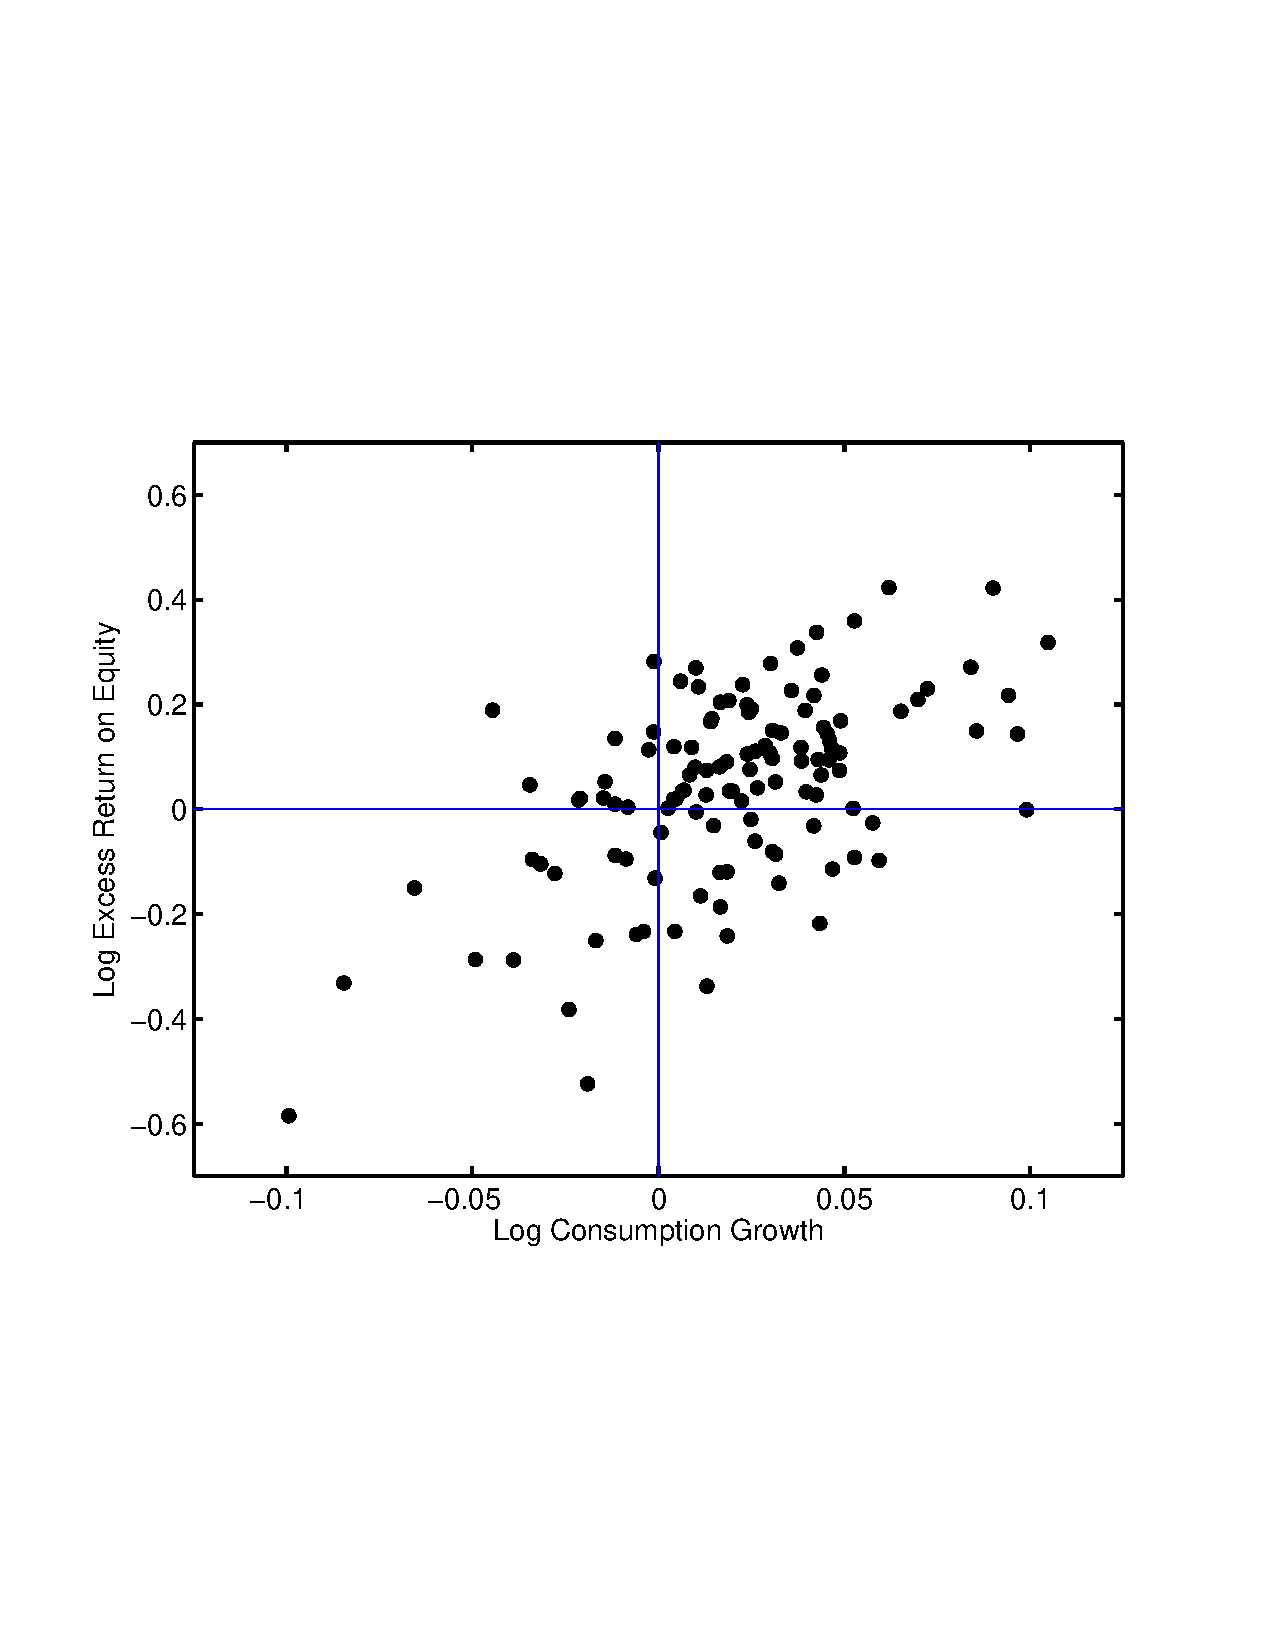
\includegraphics[width=\textwidth]{../Code/Matlab/scatter_gxr.pdf}

\vfill \centerline{\it \copyright \ \number\year \
NYU Stern School of Business}

\end{document}
